\section{The Hopfield model}
\subsection{Bitwise implementation of the Metropolis algorithm}
\begin{algorithm}[htbp]
\DontPrintSemicolon
\caption{Bitwise Hopfield Metropolis}

\KwIn{Bit-replicated spins $\{B_i\}$, couplings $\texttt{Couplings}$, neighbor lists $\partial i$, number of patterns $p$}
\KwOut{Updated spin configurations $\{B_i\}$}

\BlankLine
\textbf{Preallocated variables:}
$\mathtt{Bits}\ c_{ij},\ \mathtt{mask}$\;
$\mathtt{UnsignedInt}\ \Sigma_c,\ \Sigma_{cg},\ \Sigma_g,\ \mathrm{LHS},\ \mathrm{RHS},\ tmp$\;

\BlankLine

\For{$i=1$ \KwTo $N$}{
    $\Sigma_g(i)\leftarrow 0$\;
    \For{$j\in\partial i$}{
        $\Sigma_g(i)\mathrel{+}=G_{ij}$
    }
}
\tcp*{Precompute coupling sums}

\BlankLine

\For{$\mathrm{sweep}=1$ \KwTo $N_{\mathrm{sweeps}}$}{
    \For{$\mathrm{step}=1$ \KwTo $N$}{

        Draw a random neuron $i$\;

        Draw $q$ with $\theta \sim \mathcal{E}(2\beta/N)$\;

        \eIf{$q \geq  \Delta_k^\text{esc}$}{
            $B_i\leftarrow\neg B_i$
            \tcp*{Unconditional flip}
        }{

            $\Sigma_c\leftarrow0$\;
            $\Sigma_{cg}\leftarrow0$\;

            \For{$j\in\partial i$}{

                $c_{ij}\leftarrow B_i\odot B_j$
                \tcp*{Replica-wise agreement}

                $\Sigma_c\mathrel{+}=c_{ij}$\;

                $tmp\leftarrow G_{ij}$\;

                $tmp\leftarrow tmp\wedge c_{ij}$\;

                $\Sigma_{cg}\mathrel{+}=tmp$\;
            }

            $\mathrm{RHS}\leftarrow p\,n_i+2\,\Sigma_{cg}$\;

            $\mathrm{LHS}\leftarrow \Sigma_g(i)+r+2P\,\Sigma_c$\;

            $\mathtt{mask}\leftarrow(\mathrm{RHS}\le\mathrm{LHS})$
            \tcp*{Replica-wise acceptance test}

            $B_i\leftarrow B_i\oplus\mathtt{mask}$\;
        }
    }
}
\label{alg:Hopfield_bitwise}
\end{algorithm}
\FloatBarrier
\subsubsection{Naive implementation}
A first naive implementation would be to unfold $G_{ki}$ into its pattern components in order to deal with \Bits only objects. The flip condition would then be:

\begin{equation}
 q\geq \sum_{i \in \partial k}\sum_{\mu=1}^{p}\xi_k^\mu \xi_i^\mu S_k S_i.
\end{equation}
As seen in the previous sections, the product $\xi_k^\mu \xi_i^\mu S_k S_i$ can simply be expressed from  $X_k^\mu \odot X_i^\mu \odot B_k \odot B_i$, where $X_k^\mu$ is the boolean variable associated with $\xi_k^\mu$. This method presents the advantage to not require too much memory allocation to store the couplings $G_{ki}$ as they are not stored before the evolution but computed on the fly in the hot loop.
However, it requires summing over the patterns, thus introducing  an additional complexity of $\mathcal{O}(p)=\mathcal{O}(\alpha N)$ per spin update, which is done $N \cdot N_\text{sweeps}$ times. This would result in a significant loss of performance.

\begin{algorithm}[b]
\nolinenumbers
\DontPrintSemicolon
\caption{Bitwise Hopfield Metropolis using shifted overlaps}

\KwIn{Bit-replicated spins $\{B_i\}$, patterns $\{X_i^\mu\}$, shifted overlaps $\{\tilde{M}^\mu\}$, shifted couplings $\{\tilde{G}_{ij}\}$, neighbor lists $\partial i$, number of patterns $p$}
\KwOut{Updated spin configurations $\{B_i\}$}

\BlankLine

\textbf{Preallocated variables:}

$\mathtt{Bits}\ C_{ij},\ C_i^\mu,\ \mathtt{mask}$\;

$\mathtt{UnsignedInt}\
\Sigma_C,\
\Sigma_{CM},\
\Sigma_{CG},\
\Sigma_M,\
\mathrm{LHS},\
\mathrm{RHS}$\;

\BlankLine

\For{$\mu=1$ \KwTo $p$}{
    $\Sigma_M\leftarrow\Sigma_M+\tilde{M}^\mu$
}
\tcp*{Precompute shifted overlap sum}

\BlankLine

\For{$i=1$ \KwTo $N$}{
    $\Sigma_G(i)\leftarrow0$\;
    \For{$j\notin\partial i,\ j\neq i$}{
        $\Sigma_G(i)\leftarrow\Sigma_G(i)+\tilde{G}_{ij}$
    }
}
\tcp*{Precompute shifted non-neighbor coupling sums}

\BlankLine

\For{$\mathrm{sweep}=1$ \KwTo $N_{\mathrm{sweeps}}$}{

\For{$\mathrm{step}=1$ \KwTo $N$}{

    Draw random neuron $k$\;

    Draw $q$ with $\theta\sim\mathcal{E}(2\beta/N)$\;\;


    \eIf{$q \geq p n_k$}{

        \For{$\mu=1$ \KwTo $p$}{

            $C_k^\mu\leftarrow B_k\odot X_k^\mu$\;

            $\tilde{M}^{\mu}
            \leftarrow
            \tilde{M}^{\mu}
            +2-4C_k^\mu$\;
        }
        $\Sigma_M
        \leftarrow
        \Sigma_M
        + 2p
        - 4\sum_{\mu=1}^{p} C_k^\mu$
        \tcp*{Update shifted overlaps}
        $B_k\leftarrow\neg B_k$\;\;

    }{

        $\Sigma_C\leftarrow0$\;

        $\Sigma_{CG}\leftarrow0$\;


        \For{$i\notin\partial k,\ i\neq k$}{

            $C_{ik}\leftarrow B_i\odot B_k$\;

            $\Sigma_C\leftarrow\Sigma_C+C_{ik}$\;

            $\Sigma_{CG}
            \leftarrow
            \Sigma_{CG}
            +C_{ik}\wedge\tilde{G}_{ki}$
        }


        $\Sigma_{CM}\leftarrow0$\;

        \For{$\mu=1$ \KwTo $p$}{

            $C_k^\mu\leftarrow B_k\odot X_k^\mu$\;

            $\Sigma_{CM}
            \leftarrow
            \Sigma_{CM}
            +C_k^\mu\wedge\tilde{M}^\mu$
        }


        $\mathrm{LHS}
        \leftarrow
        q
        +2N\Sigma_C
        +\Sigma_M
        +2\Sigma_{CG}$\;


        $\mathrm{RHS}
        \leftarrow
        p n_k
        +2\Sigma_{CM}
        +\Sigma_G(k)
        +2p\Sigma_C$\;


        $\mathtt{mask}
        \leftarrow
        (\mathrm{RHS}\leq\mathrm{LHS})$
        \tcp*{Bitwise evaluation of Eq.~\eqref{eq:bitwise_flip_overlap}}


        \For{$\mu=1$ \KwTo $p$}{

            $C_k^\mu
            \leftarrow
            C_k^\mu\wedge\mathtt{mask}$\;

            $\tilde{M}^{\mu}
            \leftarrow
            \tilde{M}^{\mu}
            +2\mathtt{mask}
            -4C_k^\mu$
        }
        $\Sigma_M \leftarrow \Sigma_M
        + 2P\mathtt{mask}
        - 4\sum_{\mu=1}^{p}C_k^\mu\mathtt{mask}$\;

        $B_k
        \leftarrow
        B_k\oplus\mathtt{mask}$\;
    }
}
}
\label{alg:Hopfield_bitwise_overlaps}
\end{algorithm}
\linenumbers
\subsection{Probability of the escape condition}
With $q=\lfloor \theta \rfloor$ and $\theta \sim \mathcal{E}(\beta \kappa)$, and since $\Delta_k^\text{esc}$ is an integer, the escape probability is $P(q \geq \Delta_k^\text{esc}) = P(\theta \geq \Delta_k^\text{esc}) = e^{-\beta \kappa \Delta_k^\text{esc}}$, with $\kappa = 2/N$ in the case of the Hopfield model.
For independent random patterns, each coupling $G_{ki}=\sum_{\mu=1}^{p}\xi_k^\mu \xi_i^\mu$ is a sum of $p$ independent $\pm 1$ variables, and the couplings $G_{ki}$ of the different neighbors $i$ of $k$ are independent. The mean absolute value of such a sum is known exactly,
\begin{equation}
    \mathbb{E}\,|G_{ki}| = \frac{p}{2^{p-1}}\binom{p-1}{\lfloor (p-1)/2 \rfloor} \underset{p \gg 1}{\simeq} \sqrt{\frac{2p}{\pi}},
\end{equation}
and its variance is $p-\left(\mathbb{E}\,|G_{ki}|\right)^2 \simeq p\,(1-2/\pi)$. In each replica $r$, the sum $\sum_{i \in \partial k}|G_{ki}^{(r)}|$ therefore has mean $d_k\,\mathbb{E}|G_{ki}|$, with $d_k$ the degree of spin $k$, and fluctuations of order $\sqrt{d_k\, p}$. Taking the maximum over the $n_\text{bits}$ independent replicas shifts it by at most a few standard deviations, of order $\sqrt{2 \ln n_\text{bits}}\,\sqrt{d_k\, p\,(1-2/\pi)}$. This is a relative correction of order $\sqrt{\ln (n_\text{bits})/d_k}$, i.e. $\mathcal{O}(1/\sqrt{d_k})$ at fixed $n_\text{bits}$. To leading order, the escape threshold $\Delta_k^\text{esc}=\max_r \Bigl(\sum_{i \in \partial k}\bigl|G_{ki}^{(r)}\bigr|\Bigr)$ is thus
\begin{equation}
    \Delta_k^\text{esc} \simeq d_k \sqrt{\frac{2p}{\pi}}.
\end{equation}
With $p=\alpha N$ the number of stored patterns, this leads to the escape probability approximation:
\begin{equation}
    P_{\text{esc},k}=P\left(q \geq \Delta_k^\text{esc}\right) \sim e^{-2 \beta \frac{d_k}{N} \sqrt{\frac{2\alpha N}{\pi}}},
\end{equation}

\FloatBarrier
\subsection{Evolution of the maximum overlap of all replicas}
We show in \Cref{fig:mu_star_all_replica} the evolution of the maximum overlap $m^*$ of each of the $n_\text{bits}$ replicas, for a network of $N=1024$ neurons at $\beta=5$ and storage load $\alpha=0.03$, initialized from random states.
\nolinenumbers
\begin{figure}[htbp]
\centering
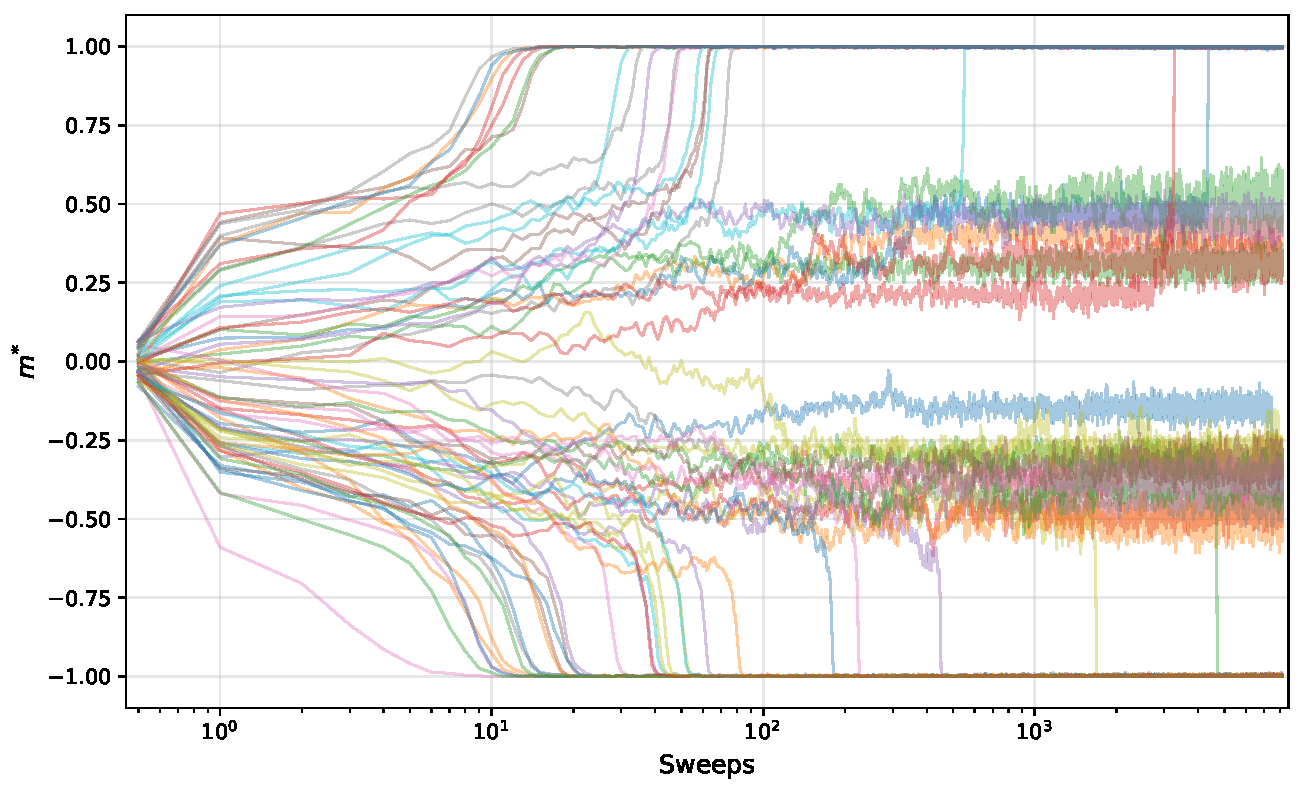
\includegraphics[width=\columnwidth]{mu_star_all_runs_N1024_beta=5.0_alpha0.030.pdf}
\caption{Evolution of the maximum overlap of each replica for $\alpha=0.03$.}
\label{fig:mu_star_all_replica}
\end{figure}
\linenumbers
